% Chapter XY

\chapter{Supplementary Data} % Main chapter title

\label{Results} % For referencing the chapter elsewhere, use \ref{Chapter2} 

% \lhead{Chapter 2. \emph{Methods}} % This is for the header on each page - perhaps a shortened title

%----------------------------------------------------------------------------------------
\section{The phosphoserine-rich N-VP2 of MVM facilitates nuclear targeting and contributes to cytotoxicity.}
\label{Cytoskeleton}


\renewcommand{\thefigure}{S\arabic{figure}}
\setcounter{figure}{0}

In order to investigate a possible involvement of the distal serine phosphorylations within N-VP2 in MVM egress, we generated a mutant, referred to as 5SG, having the corresponding serine residues substituted by glycine. In Figure~\ref{S1}, p.~\pageref{S1} several aspects of an infection with 5SG, such as cytotoxicity, nuclear targeting, and nuclear export are summarized.

\begin{figure}
\centering
  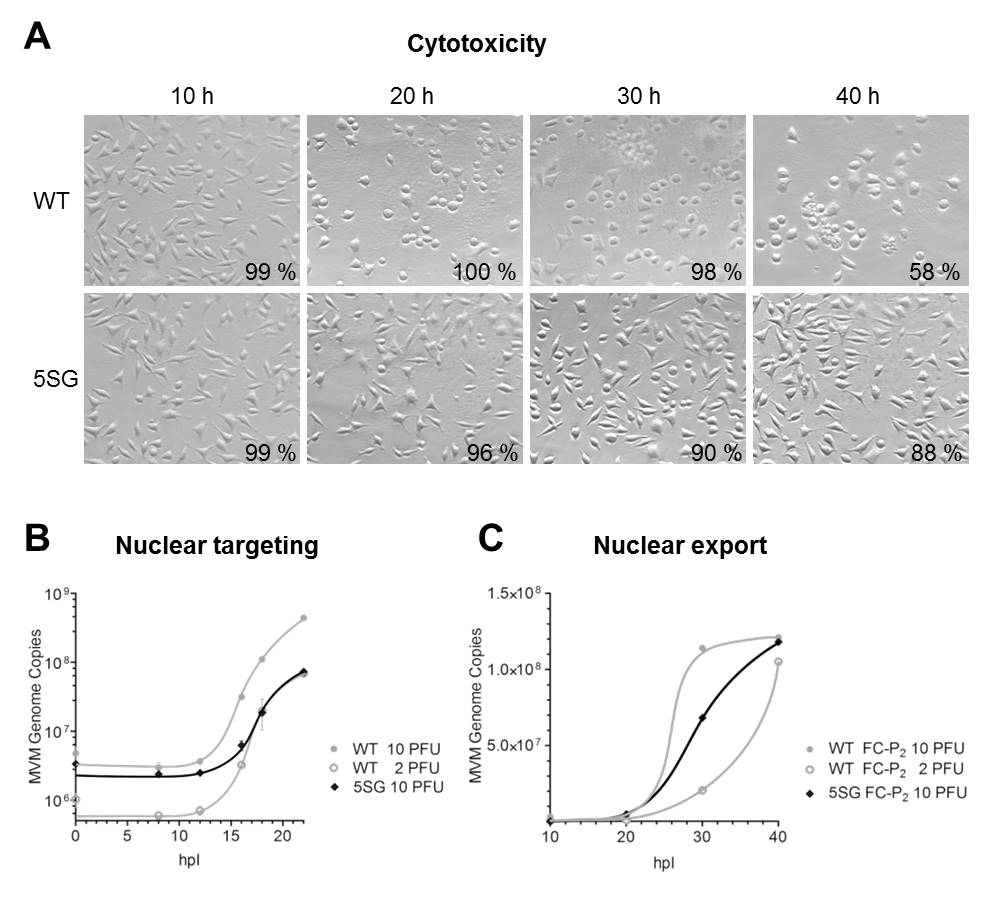
\includegraphics[scale=0.9]{S1}
  \caption[Kinetics of nuclear export depends on the input virus.]
   {\textbf{Kinetics of nuclear export depends on the input virus. (A)} A9 cells were infected with WT or 5SG MVM using 10 PFU per cell. Following binding at 4 \textcelsius~unbound virus was removed by washings. Cells were incubated at 37 \textcelsius~for the indicated times. Phase contrast pictures of the infected cells were taken using a 20$\times$ magnification objective built in a Zeiss Axiovert 35 microscope. Cell viability was accessed via trypan blue exclusion using the TC10\textsuperscript{\texttrademark} automated cell counter (BioRad). The average of three independent measurements is indicated. \textbf{(B)} A9 cells (8 $\times$ 10\textsuperscript{3}) were infected with the indicated PFU of WT or 5SG virus. Following binding at 4 \textcelsius~unbound viruses were removed. Viral DNA was extracted and quantified at the indicated times post-infection. \textbf{(C)} A9 cells (3 $\times$ 10\textsuperscript{6}) were infected using the indicated viruses and PFU. Binding was performed at 4 \textcelsius. Unbound virus was removed prior to incubation at 37 \textcelsius~for the indicated times. Cytosolic fractions were isolated and applied for AEX-qPCR. Exported FC-P\textsubscript{2} virions were quantified using qPCR. All infections were performed in the presence of $\alpha$-capsid mAb (B7) and neuraminidase in order to prevent re-infections.} 
\label{S1}
\end{figure}



In a WT infection, the cells showed reorganization of the cytoskeleton as early as 20 hpi, resulting in a rounded phenotype of affected cells. At later times, increasing amounts of cells became rounded and partially detached showing apoptotic bodies at 40 hpi, eventually resulting in cell death and cytolysis (see Figure~\ref{S1} A, 1\textsuperscript{st} row, p.~\pageref{S1}). In contrast, 5SG virions were significantly less cytotoxic. Even as late as 40 hpi most of the infected cells still exhibited the typical fibroblastic phenotype and only a few cells became rounded. No signs of apoptosis and cytolysis were observed (see Figure~\ref{S1} A, 2\textsuperscript{nd} row, p.~\pageref{S1}). 5SG was approximately 5$\times$ less efficient in replicating viral DNA in the nucleus, indicating that fewer virions reached the nucleus, thus delivering less DNA templates to initiate viral replication. Indeed, the amount of viral DNA in the nuclei of 5SG infected cells was similar to the quantities that were obtained when the cells were infected with 5$\times$ less WT virions (see Figure~\ref{S1} B, p.~\pageref{S1}). Nuclear export of 5SG progeny was not significantly affected. Virions were efficiently exported from the nucleus even though showing a slight delay in cytoplasmic accumulation (see Figure~\ref{S1} C, p.~\pageref{S1}). This delay is obviously caused by defects in early steps of infection prior to the initiation of DNA replication, such as binding, endosomal escape, viral uptake, or nuclear targeting.


As observed, productive MVM infection produces a strong cytopathic effect in the host cell, ultimately causing cellular lysis. Such dramatic changes in the cytoskeleton filaments involve gelsolin-mediated degradation of actin fibers resulting in the generation of characteristic ``actin-patches'' \cite{pmid18704167}. While the actin filaments become destabilized, the microtubule network is maintained during the course of infection \cite{pmid15582663}. The latter observation together with the previously reported capsid-dynamin co-localization~\cite{pmid18704167} would be in agreement with a microtubule dependent egress of MVM. The little delay in nuclear targeting and the fewer amount of progeny DNA in the nucleus observed for an infection with 5SG virions (see Figure~\ref{S1} B, p.~\pageref{S1}) cannot explain the considerable delay of the cytopathic effect of more than 20 h. N-VP2 is removed by proteolytic digestion during endosomal uptake. Hence, it is not involved in important signaling for replication or progeny morphogenesis. Additionally, it has been demonstrated that there are no significant differences in the cytoplasmic accumulation of WT and 5SG progeny virions (see Figure~\ref{S1} C, p.~\pageref{S1}). Therefore, the phosphorylations on N-VP2, which represent the only difference between the WT and 5SG progeny, are likely involved in late events mediating the rearrangement of the cytoskeleton during egress. 5SG seems to be defective for severing the actin filaments resulting in prolonged maintenance of the cytoskeleton and cell integrity. 


Similar observations have been reported by G. E. Tullis \textit{et al.}~\cite{pmid1448928} for a MVM mutation affecting the sequence but not the phosphorylations within N-VP2. Their results suggest that the trypsin-sensitive RVER region is important for both binding and a subsequent step prior to the onset of DNA replication. A 7 amino acid deletion mutant lacking the trypsin-sensitive residues 17-23 within N-VP2 was slightly defective for binding and approximately 10$\times$ deficient, compared to the WT, in initiating a productive infection. However, \textit{in vivo} processing of N-VP2 was still achieved. Because this mutation affects both structural proteins VP1 and VP2, it is difficult to distinguish their relative contribution to the mutant phenotype. However, the binding defect is more likely a VP2 effect since virions lacking VP1 are not defective in binding to susceptible cells \cite{pmid8416366}. In addition to its defect in cell binding, the mutant produced approximately 10$\times$ less viral DNA in the nuclei of infected cells, suggesting that fewer mutant virions, on the average, reached the nucleus where they can initiate DNA replication. Nonetheless, those that managed to reach the nucleus, replicated normally. Similar to 5SG, this mutant was delayed in egress from the cells late in asynchronous infections. However, mutant progeny virions efficiently egress early in the infection, as well as in highly synchronized infections. Therefore, this effect might be a nonspecific defect in some aspect of cytolysis rather than a defect in an active egress mechanism. A less efficient cytolysis would hamper the passive release and spread of intracellular progeny virions, thus preventing their contribution in a next round of infection.

Altogether, these results strongly suggest an involvement of N-VP2 late in infection. N-VP2 appears to orchestrate the reorganization of the cytoskeleton late in infection facilitating passive release of progeny virions. However, since early active egress remains unaffected \cite{pmid1448928}, N-VP2 does not seem to actively participate in the transport mechanism underlying active egress.        




\subsection{Isolation and characterization of empty capsids (EC)}

As previously mentioned, DNA packaging and the recently discovered capsid surface phosphorylations are a prerequisite for the externalization of N-VP2. ECs lack both a viral genome and the late phosphorylations, thus having their N-VP2 termini buried in the interior of the capsid. Therefore, EC represent an useful tool to study the role of N-VP2 during early steps in infection, such as binding and endosomal uptake. In addition to the previously characterized FC populations (FC-P\textsubscript{1} and FC-P\textsubscript{2}), infected cells also produce a considerable amount of ECs. Due to the lack of DNA, EC band at lower density compared to FC following differential centrifugation in CsCl. While FC entered the gradient to a density of 1.46 gcm\textsuperscript{-3}, EC already banded at 1.32 gcm\textsuperscript{-3}, as determined by refractometry (see Figure~\ref{S2} A, p.~\pageref{S2}). A quantitative PCR analysis of the corresponding fractions confirmed that viral DNA containing particles were depleted from ECs to almost a thousand times (see Figure~\ref{S2} B, p.~\pageref{S2}). Approximately half of the overall viral progeny population represents ECs. Therefore, it is of interest to characterize their role during the course of infection. First of all, we verified their N-VP2 conformation and the binding specificity to SA moieties. In Figure~\ref{S2} C and D, p.~\pageref{S2} it is shown that N-VP2 is not accessible to specific antibodies and proteolytic digestion by chymotrypsin (CHT), respectively. Figure~\ref{S2} E and F, p.~\pageref{S2} demonstrates that both EC and FC restrictively bind to SA moieties on the surface of murine A9 cells. Binding of both capsid species can be efficiently prevented by pre-treatment of A9 cells using neuraminidase (Neur, see Table~\ref{Enzymes}, p.~\pageref{Enzymes}) at doses higher than 50 U/mL. Neuraminidase specifically hydrolyzes glycosidic linkages of neuraminic acids. These results confirm that both capsid species bind to the same class of receptor molecules on the surface of susceptible murine cells.           


 
\renewcommand\thempfootnote{\arabic{mpfootnote}}

\begin{figure}

  \begin{minipage}{\textwidth}
\centering
  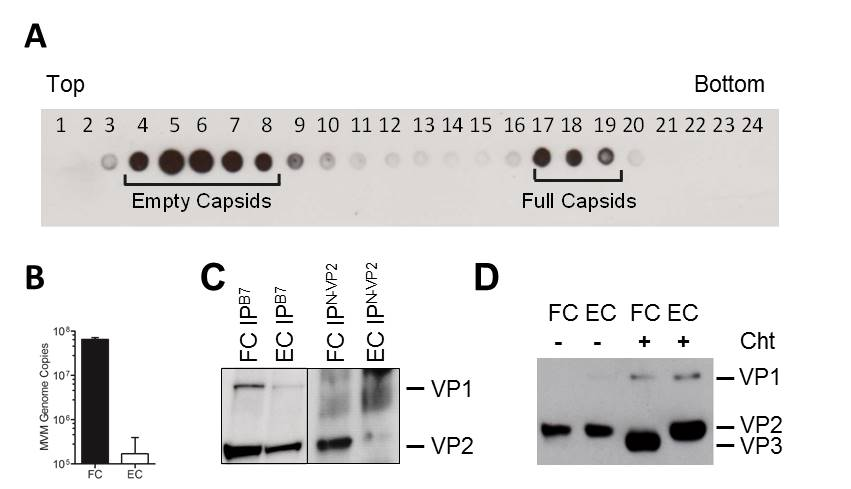
\includegraphics[scale=0.9]{S2}
  \caption[Purification and analysis of FC and EC.]
   {\textbf{Purification and analysis of FC and EC. (A)} FC and EC were separated by differential centrifugation through a CsCl gradient as described in Section~\ref{CsCl}, p.~\pageref{CsCl}. Fractions (500 $\mu$L each) are labeled from top to bottom of the gradient. 2 $\mu$L of each fraction were spotted on a nitrocellulose membrane and probed with an $\alpha$-capsid mAB (B7). A HRP-coupled secondary antibody was used and the membrane was developed by exposure to a photo film. \textbf{(B)} EC and FC fractions were pooled. qPCR analysis was performed to quantify DNA-containing particles. \textbf{(C)} N-VP2 accessibility of ECs and FCs was tested by IP using an antibody raised against the N-VP2 region. The total amount of applied viral particles was verified using an $\alpha$-capsid antibody (B7 mAb). \textbf{(D)} ECs and FCs (10\textsuperscript{8} particles each) were treated with 0.5 mg/mL chymotrypsin (CHT) or not. Proteolytic N-VP2 processing was analyzed by 10 \% SDS-PAGE. After transfer to a polyvinylidene difluoride membrane, the blot was probed with a rabbit $\alpha$-VP pAb, followed by a HRP conjugated secondary antibody. The membrane was developed by exposure to a photo film. \textbf{(E)} Following treatment with 50 U/mL neuraminidase (Neur) or not, A9 cells were infected at 4 \textcelsius~using the indicated PFU of FCs or ECs\footnotemark. Following washings to remove unbound viruses the cells were lysed in protein loading buffer and proteins were separated by 10 \% SDS-PAGE. Membranes were probed as outlined above. \textbf{(F)} Estimation of the effective dose of Neur in order to completely deplete MVM binding on A9 fibroblasts. Following neuraminidase treatment using the indicated doses, virus (5 PFU) was bound to 3 $\times$ 10\textsuperscript{5} cells for 1 h at 4 \textcelsius. Unbound virus was removed by washings, DNA was extracted and viral DNA was quantified by qPCR.} 
\label{S2}

\vspace{3cm}
\footnotetext[5]{ECs do not contain DNA and thus, they are not infectious. As a consequence, no PFUs can be calculated for ECs. FCs were quantified by qPCR analysis and used as ``external standards'' for dot blot analyses. ECs were quantified by spot densitometry by comparison to serial dilutions of quantified FCs.}

 \end{minipage}

\end{figure}





\section{Full capsids (FC) bind preferentially to murine fibroblasts}

In order to characterize the binding specificity of FC and EC, both capsid types were allowed to bind discretely to susceptible, restrictive murine fibroblasts. It was important to minimize uptake of virus into cells to exclusively study virus-receptor interactions. Viral entry can be prevented at reduced temperatures. At 4~\textcelsius, active cell-mediated uptake through endocytosis is prohibited, thus bound viral particles remain attached to their receptor molecules on the cell surface but do not internalize \cite{pmid20517}. The differences for N-VP2 accessibility can be used to distinguish FCs and ECs in IF experiments. Staining of FCs results in co-localization of $\alpha$-capsid and $\alpha$-N-VP2 antibodies whereas ECs are detected by $\alpha$-capsid antibodies only (see Figure~\ref{S3} A, upper rows, p.~\pageref{S3}). When FCs and ECs were bound to cells at equal stoichiometry, FCs preferentially bound to the cell surface, indicating a higher binding affinity for FCs compared to ECs. Co-localization of both antibodies was higher than 95 \% in the absence and in the presence of ECs. Even under non-saturated conditions, ECs were detected rarely when applied as mixed populations (see Figure~\ref{S3} A, 3\textsuperscript{rd} row, p.~\pageref{S3}). Only when an equal amount of ECs was added prior to the FCs a slight increase in bound ECs was observed. Nevertheless, ECs did not represent as much as 50 \% of the bound population but only reduced co-localization marginally to approximately 75 \% (see Figure~\ref{S3} A, lowest row, p.~\pageref{S3}). \textit{In silico} quantification of co-localization by scatter plot analysis in representative IF pictures revealed that binding of FCs was not disturbed in the presence of ECs (see Figure~\ref{S3} B, p.~\pageref{S3}). Hence, N-VP2 might assist during binding providing an advantage to cellular attachment for DNA-containing particles.            


\begin{figure}
\centering
  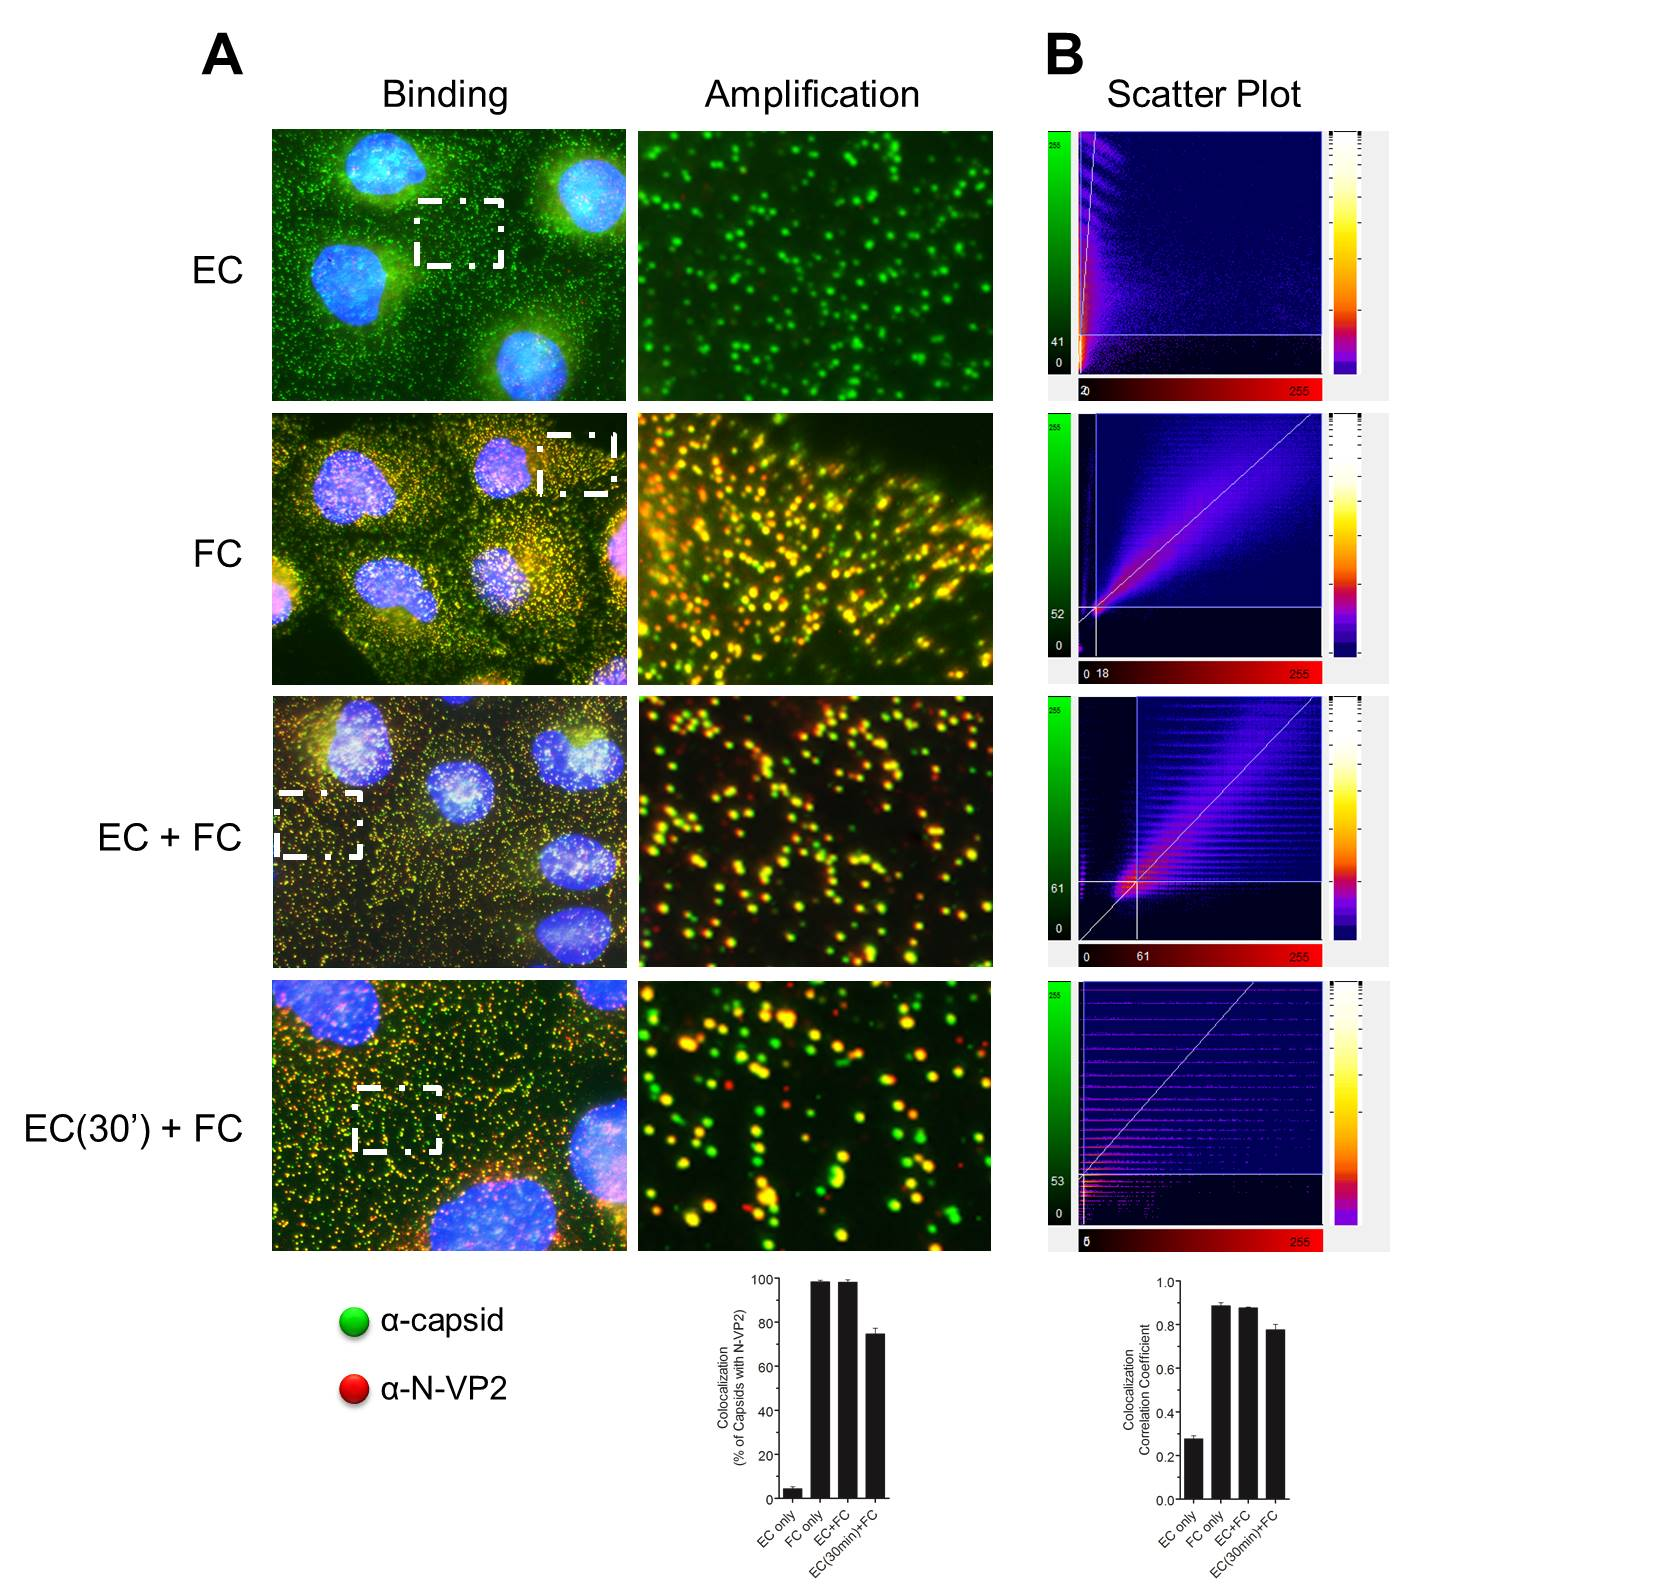
\includegraphics[width=0.95\textwidth, trim= 0mm 0mm 50mm 0mm]{S3}
  \caption[FCs are preferentially bound to the SA residues on the cell surface.]
   {\textbf{FCs are preferentially bound to the SA residues on the cell surface. (A)} A9 cells (3 $\times$ 10\textsuperscript{5}) were grown on cover slips and infected independently or combined with FC and EC (5 PFU per cell) at 4 \textcelsius. In the 4\textsuperscript{th} row ECs were incubated with the cells 30 min prior to the addition of FCs. Following removal of unbound viruses the cells were fixed and stained for IF using an antibody (mAb B7) raised against assembled capsids (green) and an antibody recognizing N-VP2 (red). Percentage of capsids showing N-VP2 signal was calculated for the indicated areas of interest. (B) Scatter plots analysis showing the indicated areas of interest were used to calculate the corresponding correlation coefficient as a measurement for the degree of co-localization.} 
\label{S3}
\end{figure}



\subsection{N-VP2 is not sufficient to provide an advantage in binding for FC}

A critical criteria for studying the attachment of a virus to its surface receptor represents the binding specificity of such an interaction. In general, specific attachment is limited to the number of available receptor molecules, thus it saturates as the amount of input virus increases. For A9 cells it has been reported that they offer 5 $\times$ 10\textsuperscript{5} specific binding sites per cell \cite{pmid20517}. In Figure~\ref{S4} A, p.~\pageref{S4} it is shown that saturation could be achieved at PFUs higher than 20, corresponding to approximately 10\textsuperscript{4} viruses per cell. In addition, specific binding can be competed by adding an excess of particles competing for the same receptor. Linser \textit{et al.} demonstrated that preliminary bound radio-labeled capsids were displaced by subsequently adding an excess of unlabeled particles. However, large quantities of unlabeled particles were required in order to demonstrate competition. Only by exceeding the amount of initially bound virus particles by 20-40$\times$, competition was observed under saturating conditions. Due to the large amount of viral particles required, they were not able to demonstrate complete competition \cite{pmid20517}. Even though working under similar conditions, we were not able to demonstrate competition between FC and EC, FC and proteolytically cleaved FC (FC\textsuperscript{CHT}), and FC\textsuperscript{CHT} and EC (see Figure~\ref{S4} B, C, and D, respectively, p.~\pageref{S4}). This indicates that still higher PFUs would have been required to demonstrate competition. However, it might be more difficult to compete for binding with EC or FC\textsuperscript{CHT} since N-VP2 might stabilize the primary attachment to the cell surface. The most clear evidence for this assumption is given by the fact that EC do not bind to the cell surface when applied together with FC as observed in IF experiments (see Figure~\ref{S3} A, lower rows, p.~\pageref{S3}). ECs might not only compete for primary receptor attachment but also for intracellular interactions required for uncoating and trafficking. Therefore, we studied the potential of EC to interfere with the progression of a natural infection. As shown in Figure~\ref{S4}, p.~\pageref{S4}, even a large excess of ECs does not interfere with the infection process. 

Altogether we conclude that ECs do not interfere with a productive infection, even though representing a large population in a normal infection. In order to disturb binding to cells, a huge excess of ECs would be required that is not found in nature. N-VP2 might be involved in the stabilization of primary attachment of MVM to susceptible cells as judged by IF analyses (see Figure~\ref{S3} A, 3\textsuperscript{rd} row, p.~\pageref{S3}). However, besides N-VP2 exposure, the packaged ssDNA genome and the surface phosphorylations represent further known differences between EC and FC which might directly or indirectly influence receptor binding. In summary, N-VP2 might have minor importance during early steps in infection except for its own proteolytic digestion which is important to allow N-VP1 externalization. However, N-VP2 appears to mediate the rearrangement of the cytoskeleton late in infection (see Section~\ref{Cytoskeleton}, p.~\pageref{Cytoskeleton}), thus being a key player in progeny egress.        



\begin{figure}
\centering
  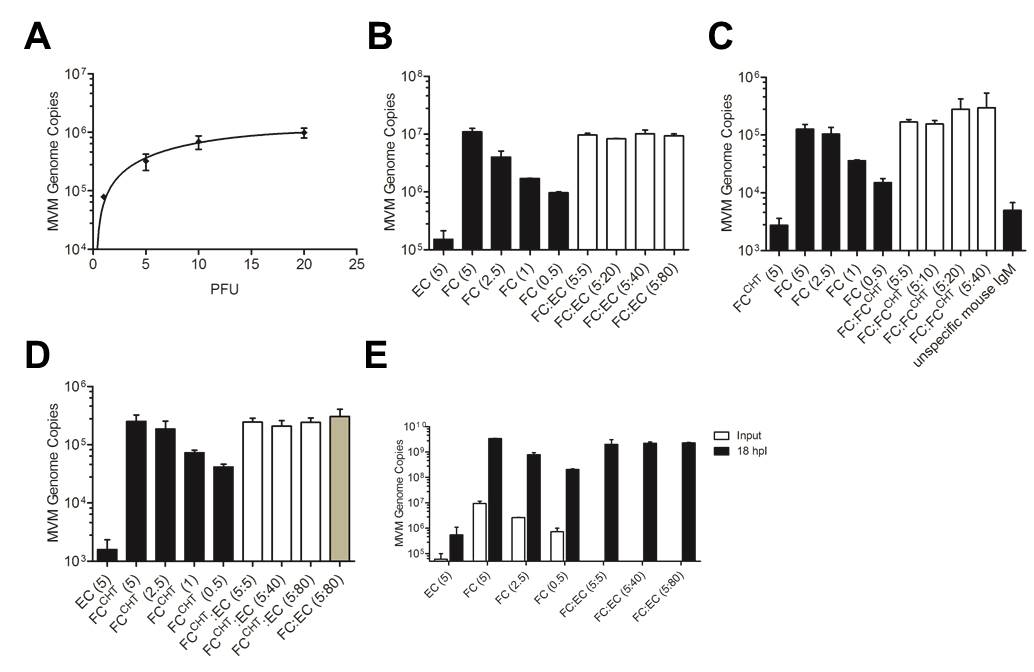
\includegraphics[scale=0.8]{S4}
  \caption[N-VP2 exposure alone is not sufficient for the better binding to SA moieties.]
   {\textbf{N-VP2 exposure alone is not sufficient for the better binding to SA moieties. (A)} A9 cells (3 $\times$ 10\textsuperscript{5}) were incubated with MVM at increasing PFU. Following binding at 4 \textcelsius~unbound virus was removed and total amount of bound virus was quantified. \textbf{(B)} ECs or FCs were bound to A9 cells at the PFUs indicated in brackets (black bars). In order to compete the bound FCs (5 PFU) increasing amounts of ECs were added (5-80 PFU, white bars). \textbf{(C)} FC\textsuperscript{CHT} or FCs were bound to A9 cells at the PFUs indicated in brackets (black bars). In order to compete the bound FCs (5 PFU) increasing amounts of FC\textsuperscript{CHT} were added (5-40 PFU, white bars). Cells were washed and lysed in cell lysis buffer (see Table~\ref{General buffers}, p.~\pageref{General buffers}). FC were quantified following IP using $\alpha$-N-VP2 Ab (see Table~\ref{Primary antibodies}, p.~\pageref{Primary antibodies}) \textbf{(D)} ECs or FC\textsuperscript{CHT} were bound to A9 cells at the PFUs indicated in brackets (black bars). In order to compete the bound FC\textsuperscript{CHT} (5 PFU) increasing amounts of ECs were added (5-80 PFU, white bars). Grey bar: As a negative control experiment, FCs (5 PFU) were simultaneously incubated with an excess of ECs (80 PFU). \textbf{(E)} A9 cells (8 $\times$ 10\textsuperscript{3}) were infected at the PFUs indicated in brackets. Increasing amount of ECs were added to FCs. Inputs are represented by white bars.} 
\label{S4}
\end{figure}










\section{Anion-exchange chromatography (AEX) can be applied on other parvoviruses}

As previously mentioned, parvoviruses undergo many interactions with their respective host cell due to their strong host cell dependence. Such interactions may preferentially occur on the very surface of incoming or progeny particles because it is readily accessible to the host's enzymes. Therefore, their net surface electrostatics can change as a consequence of host cell induced modifications on the capsid surface. As demonstrated in the present thesis, intranuclear virion populations representing different maturation stages of MVM were successfully separated by AEX based on different surface charges, in this case as a result of distinct surface phosphorylations. Fast protein liquid chromatography (FPLC, see Section~\ref{ÄKTA}, p.~\pageref{ÄKTA}) is a high performance chromatography method that combines several advantages. First, the small-diameter stationary phase enables high resolution and fast flow rates. Secondly, samples can be diluted in bio-compatible aqueous buffer systems and large sample volumes can be injected to the system. Thirdly, separation is highly reproducible due to a high level of automation including gradient program control and fraction collection. Finally, a full range of chromatography modes, such as ion exchange, chromatofocusing, gel filtration, hydrophobic interaction, and reverse phase can be provided \cite{pmid20978981}. 

We tried to apply AEX on other parvoviruses than MVM, such as B19V and CPV. B19V is a widespread human pathogen which can cause severe disease in human beings. It belongs to the genus \textit{Erythroparvovirus} (see Section~\ref{B19V}, p.~\pageref{B19V}) and thus, it is highly erythrotropic. B19V efficiently replicates in rapidly dividing erythroid progenitor cells, such as erythroblasts and megakaryocytes present in the bone marrow \cite{pmid12097253}. Only fully mature virions migrate to the blood plasma of infected individuals where they can persist at high titers (see Figure~\ref{S5} A, p.~\pageref{S5}). CPV emerged in the mid-1970s as a new pathogen of dogs. Equally to MVM, it belongs to the genus \textit{Protoparvovirus} (see Section~\ref{CPV}, p.~\pageref{CPV}) and replicates in tissues containing rapidly proliferating cells, including the bone marrow, lymph nodes, and the spleen \cite{pmid20152105}. Stocks of CPV were generated \textit{ex vivo} in canine A72 cells. The cells were productively infected and virus progeny was isolated by physical lysis of infected cell cultures. By doing so, pre-mature and mature virus progeny was not physically separated (see Figure~\ref{S5} B, p.~\pageref{S5}). 

The AEX profiles of B19V and CPV stock virus were analyzed. As expected, there was one sharp peak in the case of B19V. Since only the fully mature virions manage to migrate from the bone marrow to the blood plasma, they eluted as a single homogeneous population from the AEX column (see Figure~\ref{S5} C, p.~\pageref{S5}). On the contrary, at least two heterogeneous populations occurred in the case of CPV stock viruses that were expected to contain a mixture of several viral precursors (see Figure~\ref{S5} F, p.~\pageref{S5}). Binding interaction is known to rearrange the VP1u conformation in the case of B19V. Upon receptor attachment, B19V exposes its VP1u on the surface of its capsid \cite{pmid20826697}. Since such a rearrangement of the capsid surface influences the surface electrostatics, the profile of bound B19V was found to be distinct from the one of the stock virus (see Figure~\ref{S5} D, p.~\pageref{S5}). The situation became even more complex when intracellular virus was analyzed. B19V undergoes complex phosphorylation and partially uncoats during entry (Ruprecht, N. \textit{et al.}, manuscript in preparation). The formerly homogeneous stock virus displayed a highly complex AEX profile consisting of several peaks (see Figure~\ref{S5} D, p.~\pageref{S5}). In order to analyze such a complex profile, cell fractionation prior to AEX analysis might simplify the analysis. Another possibility would be to infect the cells in the presence of chemical compounds which interfere with certain maturation steps preventing such a complex AEX profile. 

In summary, AEX represents a powerful tool to physically separate intracellular virus populations and to gain insights into progeny virus maturation. By performing pulse chase labeling, maturation events can even be tracked chronologically.         
 






\begin{figure}
\centering
  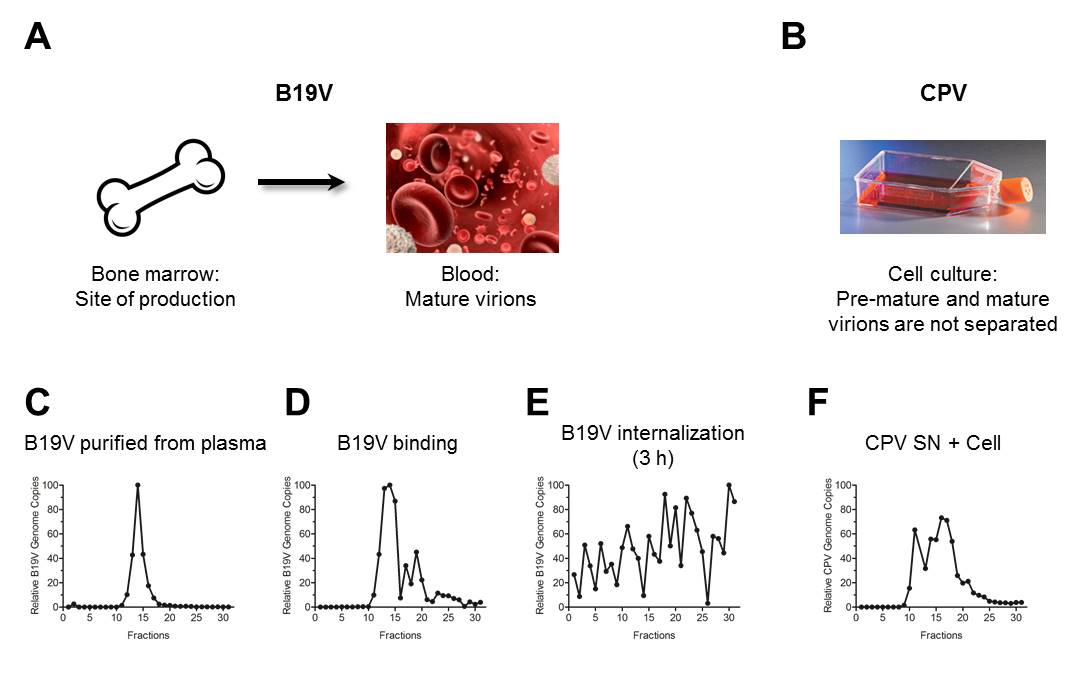
\includegraphics[scale=0.9]{S5}
  \caption[]
   {\textbf{Anion-exchange chromatography can be applied to study other parvoviruses. (A)} B19V is produced in the bone marrow of infected individuals. Only mature particles accumulate in the blood plasma where they productively infect erythroid progenitor cells. \textbf{(B)} CPV was produced in tissue cell culture. Pre-mature and mature particles were not efficiently separated. \textbf{(C)} AEX profile of B19V derived from blood plasm. \textbf{(D)} AEX profile of B19V following binding to UT-7/EPO-S1 cells at 4 \textcelsius~for 1h. \textbf{(E)} AEX profile of B19V internalized in UT-7/EPO-S1 cells for 3 h at 37 \textcelsius.  \textbf{(F)} AEX profile of CPV produced in canine A72 cells. Virus was recovered from infected cells by repeated freeze and thaw cycles to lyse the cells.} 
\label{S5}
\end{figure}





    




\renewcommand\thefigure{\thechapter.\arabic{figure}} 

